\section{Algorithms}
% TODO number of scans and slices for training and testing
The RF algorithm was trained and validated on \ldots and \ldots CT scans,
subsampled from the LIDC/IDRI database (freely available at
http://cancerimagingarchive.net/), consisting of \ldots and \ldots slices
respectively. The pixel size of the scans varied between 0,586 to 0,963 mm,
while the slice thickness varied between 1,25 or 2,5 mm. Together with the
original DICOM images the associated XML files were obtained. These XML files
provided a set of characteristics for each nodule found: region, subtlety,
spiculation, internal structure, spiculation, lobulation, shape (sphericity),
solidity, margin, and likelihood of malignancy \cite{lidcbase}.

% TODO AANTAL NODULES IN SCANS (MAX AND MIN GROOTTE?)

The LIDC/IDRI database consists of 1018 thoracic CT scans that are obtained from
a heterogeneous range of scanner models (seven GE Medical Systems LightSpeed
scanner models, four Philips Brilleance scanner models, five Siemens Definition,
Emotion, and Sensation scanner models and one Toshiba Aquilion scanner model).
The database includes only one scan per patient so the scans are not correlated.
The nodules in the scans were delineated by at least four different expert
radiologists to indentificate as much nodules as possible. For this purpose the
indentification process was also subdivided into two phases: a blinded read
phase and an unblinded read phase. During the initial blinded read phase each
radiologist independently reviewed all scans and indicated the nodules in the
range of 3 to 30 mm, the nodules smaller than 3 mm (if not clearly benign) and
the non-nodules (other pulmonary lesions e.g. an apical scar) larger or equal to
3 mm. In the subsequent unblinded read phase the anonymized blinded read results
of all radiologists were revealed to each of the radiologists who then
independently reviewed their marks along with the anonymous marks of their
colleagues. The delineation of the nodules was done completely manually or in a
semiautomated way. This was allowed as a study on this topic showed that the
variation in nodule delineation done by different radiologists
substantially exceeded the variation derived from different software tools
\cite{lidcbase}.

The initial exploration of the data and the generation of a mask to perform a
lung segmentation were done in MeVisLab 2.5.1 (VC11-64) (MeVis Medical Solutions
AG, Bremen, Germany). Further processing of the data and the implementation of
the RF algorithm were carried out in Python 2.7.6 (Python Software Foundation,
Delaware, U.S.A).  The training and testing of the RF based algorithm was
performed on a computer with Intel Core i5 CPU 1,8 GHz and 8 GB RAM. The
processing of a medium large dataset (\ldots slices) takes \ldots minutes. %
% TODO processing time

\subsection{Training of algorithm}
First the scans and the associated annotations were pre-processed in Python. The
annotations were partially provided in pixelcoordinates -- x and y values -- and
partially in worldcoordinates -- z values -- so the z coordinates were converted
into pixelcoordinates to find the nodule regions.


\subsubsection{Lung segmentation}
It was assumed that, if the whole 3D scan was fed to the cascaded
classifier, all the redundant voxels outside the lung area would be eliminated
at once. As only one feature -- the greyvalue of each voxel -- would be taken
into account on the first level of the cascaded classifier, this was not
expected to become a problem concerning memory storage. Unfortunately, it did
posed a problem so a second option was taken into consideration: a proper
lung segmentation.

By performing a lung segmentation, the amount of voxels that have to be
processed further on is significantly reduced by about 85\%. Furthermore, it has
the advantage that the soft tissues outside the lungs are eliminated so the
accuracy of the nodule detection system is increased. Therefore, it is the first
step that is performed in a lot of papers \cite{keshani, elbaz, teramoto}. We
started with implementing a lung segmentation algorithm based on \cite{keshani}.
The first part of this algorithm consists of obtaining a binary lung CT image by
adaptive fuzzy thresholding. Then two windows of different sizes are applied to
close all the gaps in the mask and the initial lung mask is obtained by sweeping
a rotated window over the entire binary image. This sweeping is necessary to
transfer non-isolated nodules into isolated ones. Finally the mask is used to
initiate an active contour model automatically for segmenting the lung area. As
stated the first step of this algorithm was supposed to provide us with a
variable, but accurate threshold to make the binary image. The performance of
this first step was assessed by applying the algorithm on 42 slices -- 28 slices
with lungs and 14 without lungs -- equally distributed over 7 scans. The results
varied among the scans. In some cases the algorithm selected the appropriate
threshold, in other cases the soft tissues around the lungs were not eliminated
well. However, a fixed threshold of 1600 emperically established to perform a
body segmentation. The lungs were eliminated from this body mask. Therefore, the
gaps (lungs) in the body maks were closed again by hole filling so a mask of the
entire body was obtained. As this body segmentation already eliminated 55\% of
all voxels and not calculations had to be done to obtain the binary image, this
results was found satisfying. Despite this reduced amount of voxels, applying
the algorithm still evoked memory errors depending on the magnitude of the scan.
% TODO tabel met experimenten om vaste threshold te bepalen er nog inzetten?

 In order to reduce the amount of voxels even further in the pre-processing
 phase, a full lung segmentation was performed in a semiautomatic way in
 MeVisLab. After the scans were uploaded in MeVisLab, the user manually
 indicates three points inside the lung area. Based on these points region
 growing is performed and a binary mask for the lung area is generated. The gaps
 in the binary mask -- which represent nodules in the lung area and nodules
 hidden in the lung wall -- are closed by dilation.
 This mask is then exported to Python for further processing of the images. An alternative way of performing a lung
 segmentation in Python would be calculating the body mask at the fixed
 threshold of 1600 and substract this mask from a similar mask but with the
 lung gaps closed. In this way only the lung area is retained. Then a dilation
 and erosion should be performed as well to include the nodules hidden in the
 lung wall.


\subsubsection{Preparation of training dataset}
Based on the associated annotations the center of gravity and the maximum radius
of each nodule was calculated. Using this information a sphere was constructed
which comprised the whole nodule. To select the central volume of the nodule,
one third of the radius was taken as an artificial boundary. Only the voxels in
this center were considered further in the process as voxels belonging to a
nodule. Reducing the amount of positive voxels -- voxels comprised by a nodule
-- was done to avoid taking into account the ambiguous edges of the nodules.
These edges might confuse the classifier. As the aim of this project was not to
delineate entire nodules but assigning nodule probabilities to the voxels in
the image, this reduction in order to provide clear training data for the
classifier was justified.

However, instead of a sphere -- which defines the nodules in 3D -- this concept
was applied per slice as it was noticed that the delineation of the nodules was
not always done properly so a lot of nodules showed a flattened shape \ref{fig:flatNodule}.
% TODO maximum of minimum radius
Therefore, the maximum radii of the nodule in each slice were separately
determined and one third of these radii was taken to select the central volume
of the nodule. A list of positive voxels per scan was constructed this way.
\begin{figure}[htp] \begin{center}   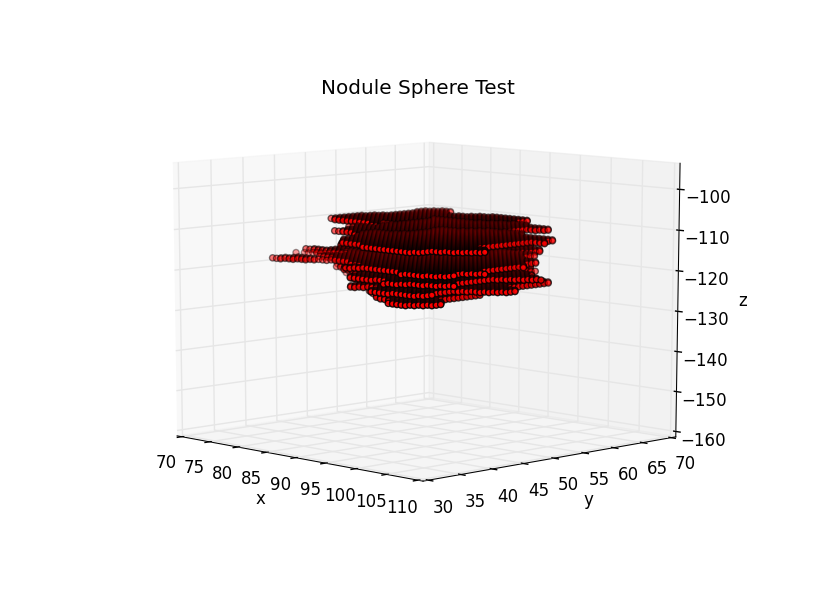
\includegraphics[width=90
mm]{img/spherenodule_001.png}   \caption{Flattened shape of nodule (LIDC scan
007)}   \label{fig:flatNodule} \end{center} \end{figure}

To train a classifier, one does not only need positive example, also negative
examples are necessary to teach the classifier. Therefore, a second list of
voxels was constructed. The amount of voxels was taken the same as in the list
of positive voxels to obtain a balanced traning dataset. The positions of the
negative voxels were selected at random over the entire image. The only
constraint was that they were not allowed the be situated within two times the
maximum radius of each nodule. This constraint was imposed to avoid ambigous
training data.

Then features were calculated for both the positive and the negative voxels. The
features that were used are discussed in \ref{sec:featureExtraction}. This
resulted in a list of features and a class (nodule or non-nodule) per voxel.
This whole process was repeated for all scans and the results were then
concatenated to obtain a dataset to train the ensemble classifier.

\subsubsection{Training Cascaded classifier}
The trainingsdataset is fed to the first level of a cascaded RF classifier. This
means that the classifier has different levels on which different amounts of
features are implemented. On a lower level, less features and less complex
features are implemented. The first feature for example is the greyvalue of each
voxel. This is a feature we get ``for free'' as they are readily available and
nothing has to be calculated. The algorithm only decides on which threshold it
uses to separate nodules from non-nodules. Using this simple feature a large
part of the voxels can already be eliminated by setting a fixed threshold.
The voxels with a probability that is lower than this threshold are considered
not to be nodules. These voxels are also removed from the trainingset and only
the remaining voxels are taken to the next level in the cascaded classifier. The
choice of the threshold is made in a empirical way. The second feature is a more
complex feature and therefore it requires more computational power. However,
this is not a problem anymore as the amount of voxels to be processed is
reduced. At the second level again a number of voxels are eliminated and removed
from the dataset. The number of levels, and therefore the number of features,
can be increased till the end results are satisfying. This however is to be
decided by the user. The classifier is organised this way as both memory and CPU
time are limited. The result of this step is the creation of a RF classifier
model. This model is then tested in the next step on new data to assess the
performance of the model.

% TODO crossvalidatie

\subsubsection{Testing Cascaded classifier}
The model that was generated in the previous step is now applied on new data to
estimate the value of the added feature in the next level of the classifier.
The question we ask ourselves here is whether a substantial amount of
non-nodule voxels are again removed from the dataset without removing the nodule
voxels as well. If this is the case the feature is kept at that level, otherwise
another feature is implemented.

The assessment is performed based on a probability image that is generated after
the model is applied on the new dataset. For each voxel in this dataset a
feature vector is calculated and this feature vector is then pushed down the
trees of the RF classifier. After each voxel is given a certain probability, the
probability image is generated.


\subsubsection{Feature extraction} \label{sec:featureExtraction}


welke features
hoe berekend

\subsection{Validation of algorithm}
nieuwe datasets van lidc ingeladen

sensitivity
specificity
FP


\subsection{Comparison with SVM}

VERGELIJKEN MET SVM?






klassendiagram: hoe is programma opgebouwd?
TRAINING + TEST
\begin{enumerate}
\item stappen die doorlopen worden + fig
\item welke algorithmes gebruikt + wat doen ze + waarom die keuze?
\item vergelijken keuzes met literatuur/commerciele systemen?
\end{enumerate}


trainingstage + teststage
tussenresultaten: moeilijkheden, opl, \ldots


